\chapter{Methodology}
\label{ch03}
This chapter discusses methodology used in this study. Firstly, the selection of Root Servers used is presented in Section \ref{ch03:root-server}. Secondly, the method used to retrieve historical BGP data is discussed in Section \ref{ch03:bgp-data}. Thirdly, types of data analysis performed and considerations taken is presented in Section \ref{ch03:analysis}.  Fourthly, visualization technique we used in Section \ref{ch03:visualization}. Finally, the concluding remarks of this chapter is provided in Section \ref{ch03:concluding}.

\section{Selecting Eligible Root Servers}
\label{ch03:root-server}
As discussed in Section \ref{ch02:dns}, there are 13 Root Servers in operation today. However, not all of them are eligible for this study. The objective of this thesis is to assess IPv4/IPv6 catchment areas of anycast service. Thus, we only select Root Servers that are anycasted and provide dual-stacked services. Among all Root Servers, we omit B and H-Root as these Roots are not anycasted yet. We also rule out E and G-Root as those are IPv4 only. Thus, it leaves us with A, C, D, F, I, J, K, L, and M-Root.

\begin{table}[h]
	\centering
	\begin{threeparttable}	
		\begin{tabular}{c c c}
			\hline
			\textbf{Root Server} & \textbf{IP Addresses}	& \textbf{IPv6 Starting Date\tnote{a}} \\ \hline\hline
			\multirow{2}{*}{A}	& 198.41.0.4	& \multirow{2}{*}{Feb 2008}  \\ & 2001:503:ba3e::2:30 \\  \hline
			
			\multirow{2}{*}{C}	& 192.33.4.12	& \multirow{2}{*}{Mar 2014}  \\ & 2001:500:2::c \\  \hline
			
			\multirow{2}{*}{D}	& 128.8.10.90, 199.7.91.13\tnote{b}	& \multirow{2}{*}{Mar 2014}  \\ & 2001:500:2d::d \\  \hline		
			
			\multirow{2}{*}{F}	& 192.5.5.241	& \multirow{2}{*}{Feb 2008}  \\ & 2001:500:2f::f \\  \hline				
			
			\multirow{2}{*}{I}	& 192.36.148.17	& \multirow{2}{*}{Jun 2010}  \\ & 2001:7fe::53 \\  \hline						
			
			\multirow{2}{*}{J}	& 192.58.128.30	& \multirow{2}{*}{Feb 2008}  \\ & 2001:503:c27::2:30 \\  \hline								
			
			\multirow{2}{*}{K}	& 193.0.14.129	& \multirow{2}{*}{Feb 2008}  \\ & 2001:7fd::1 \\  \hline	
			
			\multirow{2}{*}{L}	& 198.32.64.12, 199.7.83.42\tnote{c}	& \multirow{2}{*}{N/A}  \\ & 2001:500:3::42, 2001:500:9f::42\tnote{d} \\  
			\hline
			
			\multirow{2}{*}{M}	& 202.12.27.33	& \multirow{2}{*}{Feb 2008}  \\ & 2001:dc3::35 \\  \hline	
		\end{tabular}
		\begin{tablenotes}
			\item \url{http://www.root-servers.org/news.html}
			\item Switched to the second IP address in January 2013
			\item Switched to the second IP address in March 2016
			\item Switched to the second IP address in November 2011
		\end{tablenotes}
		\caption{Root Servers used in this thesis}
		\label{table:ch03:root-servers}
		
	\end{threeparttable}
\end{table}

Table \ref{table:ch03:root-servers} presents all Root Servers used in this study. The selected Root Servers have different starting date of dual-stack operation. Since the majority of them (A, F, H, J, K, M) started using IPv6 from February 2008\footnote{\url{http://www.iana.org/reports/2008/root-aaaa-announcement.html}}, the data analysis is started from March 1\textsuperscript{st} 2008 and ended on June 1\textsuperscript{st} 2016. The other Root Servers (C, D, I) started using IPv6 later. We cannot find information regarding L-Root's starting date. However, based on the BGP routing data, it seems L-Root started to run dual-stacked service at least in February 2008.

Root Servers use single address for each IPv4 and IPv6 for their DNS service. However, some of them changed their addresses during the observation time (second column of Table \ref{table:ch03:root-servers}). These changes are taken into account as well in our analysis program. 

\section{BGP Data Retrieval}
\label{ch03:bgp-data}
As discussed in Section \ref{ch02:measuring-anycast}, there are two projects that provide large-scale historical BGP routing data, namely RIS and RouteViews. Looking at their collector list, RouteViews\footnote{\url{http://archive.routeviews.org/}} has advantage over RIS (Table \ref{table:ch03:ris-collectors}) in terms of collectors distribution. RIS is Europe-centric, where only 6 out of 18 collectors are outside the continent and 3 of them are in USA. On the other hand, RouteViews is more globally distributed. Beyond the US and European countries, RouteViews also deploy collectors in Australia, Singapore, Nepal, and Kenya. Using both data source would be complementary. However, RouteViews only provides the raw MRT files. Typically, each collector produce \textasciitilde100 MB of BGP RIB data for each dump interval that its size keeps growing over the time. Suppose there are 17 collectors. Thus, for the time period used in this thesis (each month between March 2008 and June 2016), we should download $17 \times 100$ MB $\times  88$ months $= 149.6$ GB, not including time required to process the raw data. Due to time and resource constraints in this work, using data from RouteViews is considered to be not feasible. 

On the other hand, RIS collectors data can be accessed through RIPEStat using its API, which allows us to only access specific BGP routing information that we need. Thus, we use RIPEStat as our data provider. We specifically need to access reachability of all RIS collectors' peers in the form of AS paths to a certain prefixes, \textit{i.e.}, the Root Servers' prefixes, at a point of time. To do this, we employ data call \texttt{"BGP State"}\footnote{\url{https://stat.ripe.net/docs/data_api\#BGPState}}. We use the IP address of a Root Server as the argument, instead of its prefix. This is because some operators prefer to announce different anycast prefix lengths to distinguish global and local catchments. For instance, F-Root uses /23 prefix for its global nodes and /24 for local instances, so that routers which possess both routing information will prefer the local instances (if present) as its prefix is more specific. By using Root Server's IP addresses, we hand over the decision of which prefix chosen by the RIS peers for those addresses to the system. For example, to query BGP routing data for IPv4 prefix of M-Root on June 1\textsuperscript{st} 2016, then the following URL is used. Here the date is converted into UNIX timestamp:

\url{https://stat.ripe.net/data/bgp-state/data.json?resource=202.12.27.33&timestamp=1464739200}


\begin{table}
	\centering
	\begin{tabular}{c c c}
		\hline
		\textbf{Code} & \textbf{Location}	& \textbf{Operating Date} \\ \hline\hline
		rrc00	& RIPE NCC, Amsterdam	& Oct 1999 \\ \hline
		rrc01	& LINX, London			& Jul	 2000 \\ \hline
		rrc03	& AMS-IX and NL-IX, Amsterdam	& Jan 2001 \\ \hline
		rrc04	& CIXP, Geneva		& Apr 2001 \\ \hline
		rrc05	& VIX, Vienna		& Jun 2001 \\ \hline
		rrc06	& Otemachi, Japan	& Aug 2001 \\ \hline
		rrc07	& Stockholm, Sweden	& Apr 2002 \\ \hline
		rrc10	& Milan, Italy		& Nov 2003 \\ \hline
		rrc11	& New York (NY), USA	& Feb 2004 \\ \hline
		rrc12	& Frankfurt, Germany	& Jul 2004 \\ \hline
		rrc13	& Moscow, Russia	& Apr 2005 \\ \hline
		rrc14	& Palo Alto, USA	& Dec 2004 \\ \hline
		rrc15	& Sao Paulo, Brazil	& Dec 2005 \\ \hline
		rrc16	& Miami, USA	& Feb 2008 \\ \hline
		rrc18	& CATNIX, Barcelona	& Nov 2015 \\ \hline
		rrc19	& NAP Africa JB, Johannesburg	& Nov 2015 \\ \hline
		rrc20	& SwissIX, Zurich	& Nov 2015 \\ \hline
		rrc21	& France-IX, Paris	& Nov 2015 \\ \hline
	\end{tabular}
	\caption{List of RIS collectors used in this study}
	\label{table:ch03:ris-collectors}
\end{table}

RIPE RIS collectors gather BGP information from participating routers. These peers act as \textit{vantage points} or VPs for our measurement, and from now on we refer them simply as \textit{VPs}. VPs may have IPv4 and/or IPv6 route information towards certain Root Server. Those that possess routes to both IPv4/IPv6 prefixes of a Root Server at a given time are referred as \textit{dual-stacked VPs}. Dual-stacked VPs becomes the primary subject of this thesis since they allow us to perform comparable analysis of IPv4 and IPv6 catchments. 

\begin{figure}
	\centering
	\includegraphics[width=.6\linewidth]{img/configuration}
	\caption{Workflow of this study}
	\label{fig:ch03:config}
\end{figure}

It should be noted from Table \ref{table:ch03:ris-collectors} that the starting operation date among RIS collectors are different. This affects in the total number of the participating peers at a time. However, since the observation period is started in March 2008, the impact of new collectors addition only takes place starting in November 2015. This is particularly reflected in the notable increase of dual-stacked VPs of all Root Servers starting in the end of 2015, as can be seen later in the Chapter \ref{ch04}.

Figure \ref{fig:ch03:config} illustrates the workflow of this study. All BGP data related to Root Servers' prefixes between March 1\textsuperscript{st} 2008 and June 1\textsuperscript{st} 2016 for every first date of each month is retrieved from RIPEStat, and then persisted in two databases. Data from dual-stacked VPs that is used for data analysis is stored in MongoDB. MongoDB is selected because it is document-oriented and the data itself is in JSON format, hence makes the analysis process straightforward. Data from all VPs are stored in the second database, Neo4j, for visualization purpose. Neo4j is a graph database, hence it fits  well with the nature of BGP. It makes the queries for visualization easier. All code and data used throughout this work, including the more detailed technical description, are available at our Github repository \cite{github-thesis}.

To make the visualization informative, short description of ASes is needed. Data provided by Team Cymru Research\footnote{\url{http://www.team-cymru.org/index.html}} is used, which is accessible through their WHOIS service. Initially, we chose to perform real-time WHOIS query to provide visualization interactivity. However, sometimes Cymru does not provide quick response, which leads to poor user experience. Therefore, we decided to download AS information for all unique ASes in the database, so that the visualization front-end can quickly retrieve the data from local database. We believe that this is justified because ASN does not change much, so it is safe to have a copy in local repository.

\section{Data Analysis}
\label{ch03:analysis}

%An anycast instance is typically consisted of multiple servers for redundancy and reliability reasons. This work focuses on control-plane, thus the scope is only up to instance-level. Therefore, there is no need to identify up to server-level.


\begin{figure}
	\centering
	\includegraphics[width=.5\linewidth]{img/as-path}
	\caption{Illustration of AS path definition}
	\label{fig:ch03:as_path}
\end{figure}

The Internet can be modeled as graph, $G=(V,E)$. A vertex in $V$ represents AS, and edges in $E$ are peerings between ASes. An AS path between a source AS (\textit{i.e.}, VP of RIS) $A$ and destination AS $B$ (\textit{i.e.}, the origin AS of Root Server's prefixes)  is defined as $P_{AB}=v_0\rightarrow v_1\rightarrow v_2 \rightarrow ... \rightarrow v_{n}$ where $v_0=AS_A$, $v_{n}=AS_B$, and $n$ denotes the hop number. In this thesis, we say that $P_1$ is identical to $P_2$ if $n_1 = n_2, v_{i1}=v_{i2}$ for $i\in [0,n]$. Otherwise, $P_1$ and $P_2$ are said to have different path. In the case of $n_1 \neq n_2$, we say that $P_1$ is shorter than $P_2$ if $n_1 < n_2$.

% $\exists!v	\in(v_0, v_1, v_2, .., v_{n})$

Figure \ref{fig:ch03:as_path} illustrates AS paths relationship definition above. All paths $P_1$ to $P_5$ have origin AS $A$ and source AS $D$. $P_1$ is identical to $P_2$ since all of their transit ASes are identical. $P_1$ and $P_3$ are said to have different path even though the path lengths are similar, since there is a transit AS for a certain degree that does not identical for both of them. $P_4$ is said to have shorter path than $P_1$, and in contrary $P_5$ has longer path than $P_1$.

Networking communities use the term \textit{peering} to refer BGP session between two networks to exchange traffic between each others, typically for free. The relationship is equal for both sides. Thus, they try to keep the traffic flowing in both directions to be balanced, so that they have bargaining position to keep the connection free. Otherwise, the other party will start to charge them if their traffic is higher than their counterpart. On the other hand, the term \textit{transit} is used to describe paid BGP session between customer and provider where the provider carry all of their customer's traffic (inbound and outbound) to/from the Internet. Since it is difficult to infer the economic relationship between Root Server and their next-hop ASes based on the dataset we have, this thesis uses the term \textit{peering} broadly as its basic meaning, which is the BGP session between two BGP speakers regardless the economic cost, to refer connection between Root Servers' origin ASes with their adjacent ASes.

In this thesis, we perform comparison on IPv4 and IPv6 AS paths of a VP. If a dual-stacked VP has identical IPv4 and IPv6 paths for certain Root Server's prefixes, we refer it as \textit{converging VP}. If the paths are different, then we refer it as \textit{diverging VP}. The amount of dual-stacked VPs and converging VPs of a Root Server at a given of time is an important metric used to determine the convergence level, as discussed later (Section \ref{ch03:analysis:diff}).

To analyze the catchment areas, we address two subjects: \textit{(i)} evolution of catchment areas (Section \ref{ch03:analysis:evolution}),  and \textit{(ii)} the difference between IPv4 and IPv6 catchment areas (Section \ref{ch03:analysis:diff}). 

\subsection{Evolution of Catchment Areas}
\label{ch03:analysis:evolution}
This subject is intended to understand the AS-level dynamics due to changes made by the operators on their networks over the time. In the context of this thesis, we focus to see the dynamics in two things: \textit{(a)} the IPv4 and IPv6 networks becomes either divergent/convergent or intact, \textit{(b)} the average path lengths over the time. Thus, we use all data from VPs that possess route information towards both IPv4 and IPv6 prefixes of the Root Servers (dual-stacked VPs). 

Ideally, IPv4 and IPv6 catchment areas of a certain anycast service should be identical. In another word, IPv4 and IPv6 AS paths towards the anycast service from any given point in the Internet topology should follow the same AS hops. In this way,  IPv4 and IPv6 users experience the same path from control-plane perspective. However, this does not always the case. There are factors leading to different IPv4 and IPv6 paths towards the same destination as experienced by VPs. Firstly, the deployment of IPv6 is not as mature as IPv4 network yet. There are still some parts in the Internet that only provide IPv4 routing capabilities, especially on the Internet edges. Secondly, the network operators may have different policies or peering agreements between IPv4 and IPv6 traffic with other operators. However, Dhamdhere et al. \cite{Dhamdhere:2012:MDI:2398776.2398832} suggests that the deployment of global IPv6 network are \textit{converging} towards global IPv4 network. This can be easily understood since IPv4 network has been around for longer time and has been experiencing many optimizations and fixes of network misconfiguration, and can be considered as mature today. Thus, developing IPv6 networks based on IPv4 infrastructures will benefit from all lessons learned in the past.


To identify the convergence level of a certain anycast service (or service in general), we make use of AS path data from dual-stacked VPs. The fraction of converging VPs of all dual-stacked VPs at a time that see a Root Server's IPv4 and IPv6 prefixes is defined as the convergence level:

\begin{align*}
convergence\: level=\frac{\sum VP_{converging}}{\sum VP_{dual \: stacked}} \times 100\%
\end{align*}

%should make stronger statement for "the idea is to have shorter AS..." by re-read paper 1-hop%
Another aspect from a catchment areas evolution we are interested at is to look at the trends of average path length over the time. The idea is to have shorter AS as possible between Root Server's origin AS and the users. While short paths does not automatically guarantee better user experience (it has to be verified at data-plane level), it generally shows that the distance between two parties are likely to be close. In case of shortest path possible (direct peering), it helps in many ways \cite{Chiu:2015:WOH:2815675.2815719}:  \textit{(i)} it sidesteps potential obstacles in the form of additional transit ASes, \textit{(ii)} it allows optimal use of BGP routing policy mechanism that usually do not propagate past one hop (MED, communities), \textit{(iii)} possibility for joint traffic engineering, \textit{(iv)} prevents spoofed traffic, \textit{(v)} limits prefix hijacks, and \textit{(vi)} speeds route convergence. To understand this in the context of DNS Root service, we calculate the distribution of dual-stacked VP path lengths over the observation period to see the trends.

\subsection{The Differences Between IPv4 and IPv6 Catchment Areas}
\label{ch03:analysis:diff}
On the latter part, we focus on the differences itself as seen by the VPs. Thus, here we only use data from VPs that have different IPv4 and IPv6 paths toward a Root Server origin AS (diverging VPs). The diverging paths could happen because there are different routing policies applied for IPv4 and IPv6. For example, an operator may prefer to transit via provider \textit{A} for IPv4 connectivities to the Internet and provider \textit{B} for IPv6, perhaps due to some advantages offered by \textit{B}. One particular case is Hurricane Electric, which offer free IPv6 peering\footnote{although the traffic allowed to pass through is only for traffic with destination to Hurricane's network or its paid customers}. In fact, diverging route is a common practice we found from the datasets. This convention may results in different IPv4 and IPv6 AS path lengths experienced by the diverging VPs.

There are three aspects discussed here. \textit{Firstly}, the characterization of diverging VPs composition: how many of them experience shorter IPv4, shorter IPv6, and different paths but equal length. This information provides us illustration of an anycasted service's reachability level in IPv4 and IPv6. For example, does it really take care of its IPv6 users as its IPv4 ones? 
\textit{Secondly}, the average path lengths is again studied. Only this time for diverging VPs. Hypothetically, longer AS paths have higher probability to have diverging paths, as it will traverse more intermediate ASes with potentially diverse routing policies, compared to the short one. Longer path also means that the source AS is more likely to be located at the edge of the Internet. As we know, the IPv6 deployment in Internet edges are still lagging. Thus, IPv6 route may take sidestep to round IPv4 only networks, resulting in longer path. \textit{Thirdly}, we would like to know how different it is in terms of AS path lengths for diverging VPs. 

\section{Visualization}
\label{ch03:visualization}

A tool is developed to visualize BGP path data obtained from RIPEStat. It is web-based, so that it can be easily accessed everywhere and integrated with existing monitoring tools. D3.js \cite{d3js}, a JavaScript library for manipulating documents based on data, is used at the front-end to render the graph due to its powerful and rich visualization types. To feed the visualization data, a back-end application based on Flask is developed, which accesses the databases described in Section \ref{ch03:bgp-data}.
%In CAIDA's AS core visualization, the center of the graph are ASes with high transit degree. In contrast to this, our graph resembles a tree, with the root of the tree is the Root Server's AS(es).

The tool is developed based on work result from \cite{github-anycast} (Section \ref{ch02:visualization}). One fundamental difference is the use of forced layout instead of radial Reingold-Tilford tree as used by the authors. While the latter one is excellent on arranging ASes based on their AS path level relative to the origin AS, it constructs the visualization based on each individual VP's AS path. Thus, the transit ASes might be visually duplicated in other part of the graph and does not provide complete picture of the catchment. Forced layout eliminates this by removing hierarchical display and provides visualization as a whole AS interconnections. To compensate the lack of AS path level information, we use color code to group ASes with the same AS path level. To simplify the visualization, AS prepending property is encoded as the thickness of the line connecting two ASes, instead of repeatedly displaying the same AS as sequence of nodes.

Further improvement is made by providing interactivity. Graph can be selected for any particular point of time in the observation period. To allow operator performing comparison, IPv4 and IPv6 catchment areas are displayed side by side with the list of mutual dual-stacked VPs presented below. As the network can grow quite large and complex, the graph elements can be zoomed in and out, panned, and moved for better readability. To make the IPv4/IPv6 path comparison of a certain dual-stacked VPs easier, both IPv4 and IPv6 AS paths are highlighted when it is hovered. The short AS description retrieved from Team Cymru is also displayed on top of it.

\section{Concluding Remarks}
\label{ch03:concluding}
Not all Root Servers can be used in this study because non-anycasted and IPv4-only are excluded. For the data provider, using both RIS and RouteViews would be complementary because they cover different collector placements. However, due to constraints in this work, only RIS is used since it provides easy access to their historical BGP data. Then, some definitions used in the upcoming analysis is described in Section \ref{ch03:analysis}. The subjects of analysis are also presented, covering evolution of catchment areas and the differences between IPv4 and IPv6 catchments itself. Finally, for the visualization, we extend the work from \cite{github-anycast} with a change graph type and improvements in visualization interactivity.